\documentclass{article}
\usepackage[utf8]{inputenc}
\usepackage[T1]{fontenc}
\usepackage[paperwidth=5in, margin=1cm]{geometry}
\usepackage[export]{adjustbox}
\usepackage{wrapfig}
\usepackage{menukeys}

\usepackage{lmodern}

\newcommand\ToXinB{\mbox{%
    \raisebox{0.4pt}{T}\hspace{-1pt}\raisebox{1pt}{o}%
    \hspace{-1.6pt}X\hspace{-1pt}{\itshape in}}}

\newcommand\ToXin{\mbox{%
    \raisebox{0.5pt}{T}\hspace{-.8pt}\raisebox{1pt}{o}%
    \hspace{-1pt}X{\hspace{-1pt}\itshape in}}}

\newcommand\keyplus{\raisebox{.7pt}{\fontsize{8}{8}\selectfont+}}
\newcommand\myreturn{\fontsize{9}{9}\selectfont\return}

\newcommand\smiley{\raisebox{-1.3pt}{
\includegraphics[width=.85em]{gfx/smiley.png}}}

\begin{document}

\section*{\ToXinB: Online \LaTeX\ System\hfill

\includegraphics[width=1cm,valign=t]{gfx/leaf.png}~
}

Welcome to \ToXin! 

\bigskip\noindent
{\ToXin} allows you to compose {\LaTeX} documents in your browser, typeset them,
and edit them easily with modern Sync{\TeX} support.

\bigskip\noindent
Everything runs on your browser platform ---
\textbf{there is no server!!}

\bigskip\noindent
If this is your first time using {\ToXin},
try this:

\begin{itemize}
\item Click the crossed hammers icon
 (
\includegraphics[width=12pt,valign=t]{gfx/button-build.png}).
 This will build the current project,
 which is, by default, \textsf{scientific-writing-exercise} (from Overleaf). \\[.2em]
 \textit{The resulting PDF will be shown in this pane. To come back here to the manual, press {\rm F1}.}\\[.2em]
 \textit{To show the compiled document again, press {\rm Esc}.}

 
\item Zoom in and out using pinch or Ctrl{\,\keyplus\,}mouse wheel.
To move between pages, click the white area of the page to move the focus there,
then use either $\leftarrow$/$\rightarrow$
or PgUp/PgDn.
 
\item Move the mouse cursor over text lines in the compiled PDF.
{\ToXin} highlights lines and formula parts in green.
Click an element to jump to the corresponding line in the {\LaTeX} source editor.

\item When in the editor, press Ctrl\keyplus Enter ({\cmd\keyplus\myreturn\,} on a Mac keyboard).
The correponding line is shown in blue in the PDF.
Press the key combination twice to enable \emph{line tracking}: the blue mark will move in concert with where the cursor is in the editor.
Press Esc to exit tracking mode.

\item 
\begin{minipage}[t]{4in}
~
\begin{wrapfigure}[7]{r}{3cm}
\vspace{-3.2em}
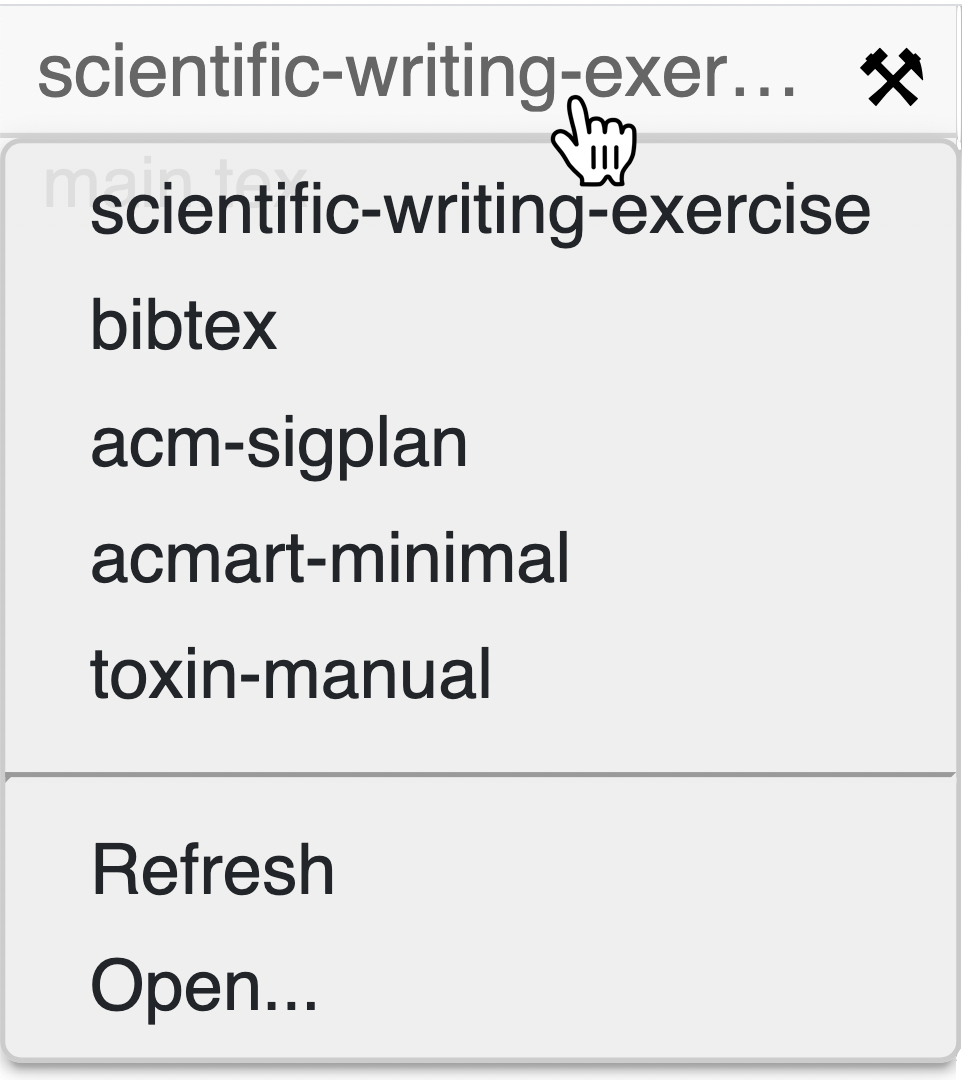
\includegraphics[width=3cm]{gfx/project-dropdown.png}
\end{wrapfigure}
\vspace{-2.4em}

Browse sample projects by clicking the project header.
Notice that only a fraction of the existing
{\LaTeX} packages is currently available;
more will be enabled in the future.
Notably, the official example of the
\texttt{acmart} class is included (as well as this manual \smiley).
\end{minipage}


\end{itemize}


\end{document}